% -- \include{b2uincl.tex}
% ======================================================================
\subsection{Inclusive CKM-suppressed decays}
\label{slbdecays_b2uincl}
% ----------------------------------------------
The large background from $\B\to X_c\ell^+\nul$ decays is the chief
experimental limitation in determinations of $\vub$.  Cuts designed to
reject this background limit the acceptance for $\B\to X_u\ell^+\nul$
decays. The calculation of partial rates for these restricted
acceptances is more complicated and requires substantial theoretical machinery.
In this update, we use several theoretical calculations
to extract \vub. We do not advocate the use of one method over another.
The authors for the different calculations have provided 
codes to compute the partial rates in limited regions of phase space covered by the measurements. 
Latest results by Belle~\cite{ref:belle-multivariate} and \babar~\cite{ref:babar-finalupdate} 
explore bigger and bigger portions of phase space, with a consequent reduction of the theoretical 
uncertainties. 

For the averages we performed, the systematic errors associated with the
modeling of $\B\to X_c\ell^+\nul$ and $\B\to X_u\ell^+\nul$ decays and the theoretical
uncertainties are taken as fully correlated among all measurements.
Reconstruction-related uncertainties are taken as fully correlated within a given experiment.
We use all results published by \babar\ in~\cite{ref:babar-finalupdate}, since the 
statistical correlations are given. 
To make use of the theoretical calculations of Ref.~\cite{ref:BLL}, we restrict the
kinematic range in $M_X$ and $q^2$, thereby reducing the size of the data
sample significantly, but also the theoretical uncertainty, as stated by the
authors~\cite{ref:BLL}.
The dependence of the quoted error on the measured value for each source of error
is taken into account in the calculation of the averages.
Measurements of partial branching fractions for $\B\to X_u\ell^+\nul$
transitions from $\Upsilon(4S)$ decays, together with the corresponding accepted region, 
are given in Table~\ref{tab:BFbulnu}.  
The signal yields for all the measurements shown in Table~\ref{tab:BFbulnu}
are not rescaled to common input values of the $B$ meson lifetime (see Sect.~\ref{sec:life_mix})
%  replace with PDG_2008 which is in EndOfYear2011.bib 
% and the semileptonic width~\cite{PDG_2007}.
and the semileptonic width~\cite{PDG_2008}.

It has been first suggested by Neubert~\cite{Neubert:1993um} and later detailed by Leibovich, 
Low, and Rothstein (LLR)~\cite{Leibovich:1999xf} and Lange, Neubert and Paz (LNP)~\cite{Lange:2005qn}, 
that the uncertainty of
the leading shape functions can be eliminated by comparing inclusive rates for
$\B\to X_u\ell^+\nul$ decays with the inclusive photon spectrum in $\B\to X_s\gamma$,
based on the assumption that the shape functions for transitions to light
quarks, $u$ or $s$, are the same to first order.
However, shape function uncertainties are only eliminated at the leading order
and they still enter via the signal models used for the determination of efficiency. 
For completeness, we provide a comparison of the results using 
calculations with reduced dependence on the shape function, as just
introduced, with our averages using different theoretical approaches.
Results are presented by \babar\ in Ref.\cite{Aubert:2006qi} using the LLR prescription. 
In another work (Ref.~\cite{Golubev:2007cs}), \vub\ was extracted from the 
endpoint spectrum of $\B\to X_u\ell^+\nul$ from \babar~\cite{ref:babar-endpoint}, 
using several theoretical approaches with reduced dependence on the shape function.
In both cases, the photon energy spectrum in the 
rest frame of the $B$-meson by \babar~\cite{Aubert:2005cua} has been used.


\begin{table}[!htb]
\caption{\label{tab:BFbulnu}
Summary of inclusive determinations of partial branching
fractions for $B\rightarrow X_u \ell^+ \nu_{\ell}$ decays.
The errors quoted on $\Delta\cbf$ correspond to
statistical and systematic uncertainties.
%%%%The statistical correlations between the analysis are given where applicable. 
The $s_\mathrm{h}^{\mathrm{max}}$ variable is described in Refs.~\cite{ref:shmax,ref:babar-elq2}. }
\begin{center}
\begin{small}
\begin{tabular}{|llcl|}
\hline
Measurement & Accepted region &  $\Delta\cbf [10^{-4}]$ & Notes\\
\hline\hline
CLEO~\cite{ref:cleo-endpoint}
& $E_e>2.1\,\gev$ & $3.3\pm 0.2\pm 0.7$ &  \\ 
\babar~\cite{ref:babar-elq2}
%%%%CB PUT NEW PREL BABAR& $E_e>2.0\,\gev$, $s_\mathrm{h}^{\mathrm{max}}<3.5\,\mathrm{GeV^2}$ & $4.4\pm 0.4\pm 0.4$ & \\
& $E_e>2.0\,\gev$, $s_\mathrm{h}^{\mathrm{max}}<3.5\,\mathrm{GeV^2}$ & $4.0\pm 0.2\pm 0.3$ & \\
\babar~\cite{ref:babar-endpoint}
& $E_e>2.0\,\gev$  & $5.7\pm 0.4\pm 0.5$ & \\
Belle~\cite{ref:belle-endpoint}
& $E_e>1.9\,\gev$  & $8.5\pm 0.4\pm 1.5$ & \\
\babar~\cite{Lees:2011fv}
& $M_X<1.7\,\gev/c^2, q^2>8\,\gev^2/c^2$ & $6.9\pm 0.6\pm 0.4$ & 
%(52\%,46\%) correlation with \babar\ ($p^*_{\ell} > 1 \gev/c$, $p^*_{\ell} > 1.3 \gev/c$) analyses
\\
Belle~\cite{ref:belle-mxq2Anneal}
& $M_X<1.7\,\gev/c^2, q^2>8\,\gev^2/c^2$ & $7.4\pm 0.9\pm 1.3$ & \\
Belle~\cite{ref:belle-mx}
& $M_X<1.7\,\gev/c^2, q^2>8\,\gev^2/c^2$ & $8.5\pm 0.9\pm 1.0$ & used only in BLL average\\
\babar~\cite{Lees:2011fv}
& $P_+<0.66\,\gev$  & $9.9\pm 0.9\pm 0.8 $ & 
%%(46\%, 78\%, 61\%) correlations with \babar\ ($(M_X-q^2)$, $p^*_{\ell} > 1 \gev/c$, $p^*_{\ell} > 1.3 \gev/c$) 
%% analyses
\\
%%%%BELLE~\cite{ref:belle-mx}
%%%%& $P_+<0.66\,\gev$  & $11.0\pm 1.0\pm 1.6$ & not used in averages\\ 
\babar~\cite{Lees:2011fv}
& $M_X<1.7\,\gev/c^2$ & $11.6\pm 1.0\pm 0.8 $ &
%%(86\%, 55\%, 94\%, 73\%) correlations with \babar\ ($P_+$, $(M_X-q^2)$,
%%$p^*_{\ell} > 1 \gev/c$, $p^*_{\ell} > 1.3 \gev/c$)  analyses 
\\ 
\babar~\cite{Lees:2011fv}
& $M_X<1.55\,\gev/c^2$ & $10.9\pm 0.8\pm 0.6 $ & 
%%(74\%, 77\%, 50\%, 72\%, 57\%) correlations with \babar\ ($P_+$, $M_X<1.7\,\gev/c^2$, $(M_X-q^2)$, 
%%$p^*_{\ell} > 1 \gev/c$, $p^*_{\ell} > 1.3 \gev/c$)  analyses 
\\ 
%%%%BELLE~\cite{ref:belle-mx}
%%%%& $M_X<1.7\,\gev/c^2$ & $12.3\pm 1.1\pm 1.2$ & not used in averages\\ 
Belle~\cite{ref:belle-multivariate}
& $p^*_{\ell} > 1 \gev/c$ & $19.6\pm 1.7\pm 1.6$ & \\
\babar~\cite{Lees:2011fv}
& ($M_X, q^2$) fit, $p^*_{\ell} > 1 \gev/c$  & $18.2\pm 1.3\pm 1.5$ & 
%%74\% correlation with $p^*_{\ell} > 1.3 \gev/c$ analysis\\ \hline
\\ 
\babar~\cite{Lees:2011fv}
& $p^*_{\ell} > 1.3 \gev/c$  & $15.5\pm 1.3\pm 1.4$ & 
%%67\% correlation with \babar\ $P_+$ analysis 
\\ \hline
\end{tabular}\\
\end{small}
\end{center}
\end{table}



\subsubsection{BLNP}
Bosch, Lange, Neubert and Paz (BLNP)~\cite{ref:BLNP,
% removed missing reference TJG 13/5/2012
%  ref:Neubert-new-1,ref:Neubert-new-2,ref:Neubert-new-3,ref:Neubert-new-4}
  ref:Neubert-new-1,ref:Neubert-new-2,ref:Neubert-new-3}
provide theoretical expressions for the triple
differential decay rate for $B\to X_u \ell^+ \nul$ events, incorporating all known
contributions, whilst smoothly interpolating between the 
``shape-function region'' of large hadronic
energy and small invariant mass, and the ``OPE region'' in which all
hadronic kinematical variables scale with the $b$-quark mass. BLNP assign
uncertainties to the $b$-quark mass which enters through the leading shape function, 
to sub-leading shape function forms, to possible weak annihilation
contribution, and to matching scales. 
The BLNP calculation uses the shape function renormalization scheme; the heavy quark parameters determined  
from the global fit in the kinetic scheme, described in \ref{globalfitsKinetic}, were therefore 
translated into the shape function scheme by using a prescription by Neubert 
\cite{Neubert:2004sp,Neubert:2005nt}. The resulting parameters are 
$m_b(SF)=(4.569 \pm 0.023 \pm 0.011)$ GeV, 
$\mu_\pi^2(SF)=(0.145 \pm 0.089 ^{+0.020}_{-0.040})$ GeV$^2$, 
where the second uncertainty is due to the scheme translation. 
The extracted values of \vub\, for each measurement along with their average are given in
Table~\ref{tab:bulnu} and illustrated in Figure~\ref{fig:BLNP}. 
The total uncertainty is $^{+5.7}_{-5.9}\%$ and is due to:
statistics ($^{+2.0}_{-2.1}\%$),
detector ($^{+1.8}_{-1.9}\%$),
$B\to X_c \ell^+ \nul$ model ($^{+1.2}_{-1.2}\%$),
$B\to X_u \ell^+ \nul$ model ($^{+1.8}_{-1.7}\%$),
heavy quark parameters ($^{+2.4}_{-2.4}\%$),
SF functional form ($^{+0.2}_{-0.3}\%$),
sub-leading shape functions ($^{+0.6}_{-0.7}\%$),
BLNP theory: matching scales $\mu,\mu_i,\mu_h$ ($^{+3.8}_{-3.8}\%$), and
weak annihilation ($^{+0.0}_{-1.5}\%$).
The error on the HQE parameters ($b$-quark mass and $\mu_\pi^2)$ 
is the source of the largest uncertainty, while the
uncertainty assigned for the matching scales is a close second. The uncertainty due to 
weak annihilation has been assumed to be asymmetric, i.e. it only tends to decrease \vub.

\begin{table}[!htb]
\caption{\label{tab:bulnu}
Summary of input parameters used by the different theory calculations,
corresponding inclusive determinations of $\vub$ and their average.
The errors quoted on \vub\ correspond to
experimental and theoretical uncertainties, respectively.}
\begin{center}
\resizebox{0.99\textwidth}{!}{
\begin{tabular}{|lccccc|}
\hline
 & BLNP &DGE & GGOU & ADFR &BLL \\
\hline\hline
\multicolumn{6}{|c|}{Input parameters}\\ \hline
scheme & SF           & $\overline{MS}$ & kinetic &  $\overline{MS}$ & $1S$ \\ 
Ref.       & \cite{Neubert:2004sp,Neubert:2005nt} & Ref.~\cite{PDG_2010} & 
see Sec.~\ref{globalfitsKinetic}  & Ref.~\cite{PDG_2010} & Ref.~\cite{Barberio:2008fa} \\
%%%%%       & (only $b\to c \ell\nu$ & & ($b\to c \ell\nu$ + $b\to s\gamma$ &  & \\
%%%%%       & moments) & & moments) & &  \\
$m_b$ (GeV)           & 4.569 $\pm$ 0.025 & 4.177 $\pm 0.043$ & 4.541 $\pm 0.023$ & 4.177 $\pm 0.043$ & 4.704 $\pm 0.029$ \\
$\mu_\pi^2$ (GeV$^2$) & 0.145 $^{+0.091}_{-0.097}$ & -                 & 0.414 $\pm 0.078$ & - &  - \\
\hline\hline
Ref. & \multicolumn{5}{c|}{$|V_{ub}|$ values}\\ 
\hline
$E_e$~\cite{ref:cleo-endpoint} &
$4.28\pm 0.50 ^{+0.31}_{-0.36}$ &
$3.90\pm 0.45 ^{+0.26}_{-0.28}$ &
$4.21\pm 0.49 ^{+0.23}_{-0.33}$ &
$3.44\pm 0.40 ^{+0.16}_{-0.16}$ &
- \\

$M_X, q^2$~\cite{ref:belle-mxq2Anneal}&
$4.49\pm 0.47 ^{+0.28}_{-0.30}$ &
$4.46\pm 0.47 ^{+0.20}_{-0.22}$ &
$4.50\pm 0.47 ^{+0.28}_{-0.31}$ &
$3.94\pm 0.41 ^{+0.17}_{-0.17}$ &
$4.68\pm 0.49 ^{+0.30}_{-0.30}$ \\

$E_e$~\cite{ref:belle-endpoint}&
$4.93\pm 0.46 ^{+0.27}_{-0.29}$ &
$4.85\pm 0.45 ^{+0.21}_{-0.25}$ &
$4.93\pm 0.46 ^{+0.17}_{-0.22}$ &
$4.50\pm 0.42 ^{+0.20}_{-0.20}$ &
-\\

$E_e$~\cite{ref:babar-endpoint}&
$4.54\pm 0.26 ^{+0.27}_{-0.33}$ &
$4.34\pm 0.25 ^{+0.23}_{-0.25}$ &
$4.50\pm 0.26 ^{+0.18}_{-0.25}$ &
$3.94\pm 0.22 ^{+0.20}_{-0.19}$ &
-\\

$E_e,s_\mathrm{h}^{\mathrm{max}}$~\cite{ref:babar-elq2}&
$4.53\pm 0.22 ^{+0.33}_{-0.38}$ &
$4.17\pm 0.20 ^{+0.28}_{-0.29}$ &
- &
$3.64\pm 0.18 ^{+0.17}_{-0.17}$ &
%%%%%%%?!?!?!?!?$4.71\pm 0.50 ^{+0.35}_{-0.35}$ \\
 \\ 

$p^*_{\ell}$~\cite{ref:belle-multivariate}&
$4.49\pm 0.27 ^{+0.20}_{-0.22}$ &
$4.63\pm 0.28 ^{+0.13}_{-0.13}$ &
$4.60\pm 0.27 ^{+0.10}_{-0.11}$ &
$4.52\pm 0.30 ^{+0.19}_{-0.19}$ &
- \\

$M_X$~\cite{Lees:2011fv}&
$4.30\pm 0.20 ^{+0.28}_{-0.27}$ &
$4.53\pm 0.21 ^{+0.24}_{-0.22}$ &
$4.29\pm 0.20 ^{+0.21}_{-0.22}$ &
$3.84\pm 0.18 ^{+0.19}_{-0.19}$ &
- \\
$M_X$~\cite{Lees:2011fv}&
$4.04\pm 0.22 ^{+0.23}_{-0.23}$ &
$4.26\pm 0.24 ^{+0.26}_{-0.24}$ &
$4.09\pm 0.23 ^{+0.18}_{-0.19}$ &
$3.76\pm 0.21 ^{+0.18}_{-0.17}$ &
- \\

$M_X,q^2$~\cite{Lees:2011fv}&
$4.30\pm 0.23 ^{+0.26}_{-0.28}$  &
$4.27\pm 0.22 ^{+0.20}_{-0.20}$  &
$4.32\pm 0.23 ^{+0.27}_{-0.30}$  &
$3.76\pm 0.20 ^{+0.17}_{-0.16}$  &
$4.50\pm 0.24 ^{+0.29}_{-0.29}$ \\

$P_+$~\cite{Lees:2011fv}&
$4.15\pm 0.25 ^{+0.28}_{-0.27}$  &
$4.24\pm 0.26 ^{+0.37}_{-0.32}$  &
$4.24\pm 0.26 ^{+0.32}_{-0.32}$  &
$3.59\pm 0.22 ^{+0.19}_{-0.18}$  &
- \\

$p^*_{\ell}$, $(M_X,q^2)$ fit~\cite{Lees:2011fv}&
$4.32\pm 0.24 ^{+0.19}_{-0.21}$  &
$4.46\pm 0.24 ^{+0.13}_{-0.13}$  &
$4.42\pm 0.24 ^{+0.09}_{-0.11}$  &
$4.35\pm 0.24 ^{+0.18}_{-0.18}$  &
- \\

$p^*_{\ell}$~\cite{Lees:2011fv}&
$4.32\pm 0.27 ^{+0.20}_{-0.21}$  &
$4.44\pm 0.27 ^{+0.15}_{-0.14}$  &
$4.41\pm 0.27 ^{+0.10}_{-0.12}$  &
$4.30\pm 0.27 ^{+0.19}_{-0.18}$  &
- \\

$M_X,q^2$~\cite{ref:belle-mx}&
- &
- &
- &
- &
$5.01\pm 0.39 ^{+0.32}_{-0.32}$ \\
\hline
Average &
$4.45\pm 0.16 ^{+0.21}_{-0.22}$ &
$4.52\pm 0.16 ^{+0.15}_{-0.16}$ &
$4.51\pm 0.16 ^{+0.12}_{-0.15}$ &
$4.05\pm 0.13 ^{+0.18}_{-0.11}$ &
$4.62\pm 0.20 ^{+0.29}_{-0.29}$ \\
\hline
\end{tabular}
}
\end{center}
\end{table}


\begin{figure}
\begin{center}
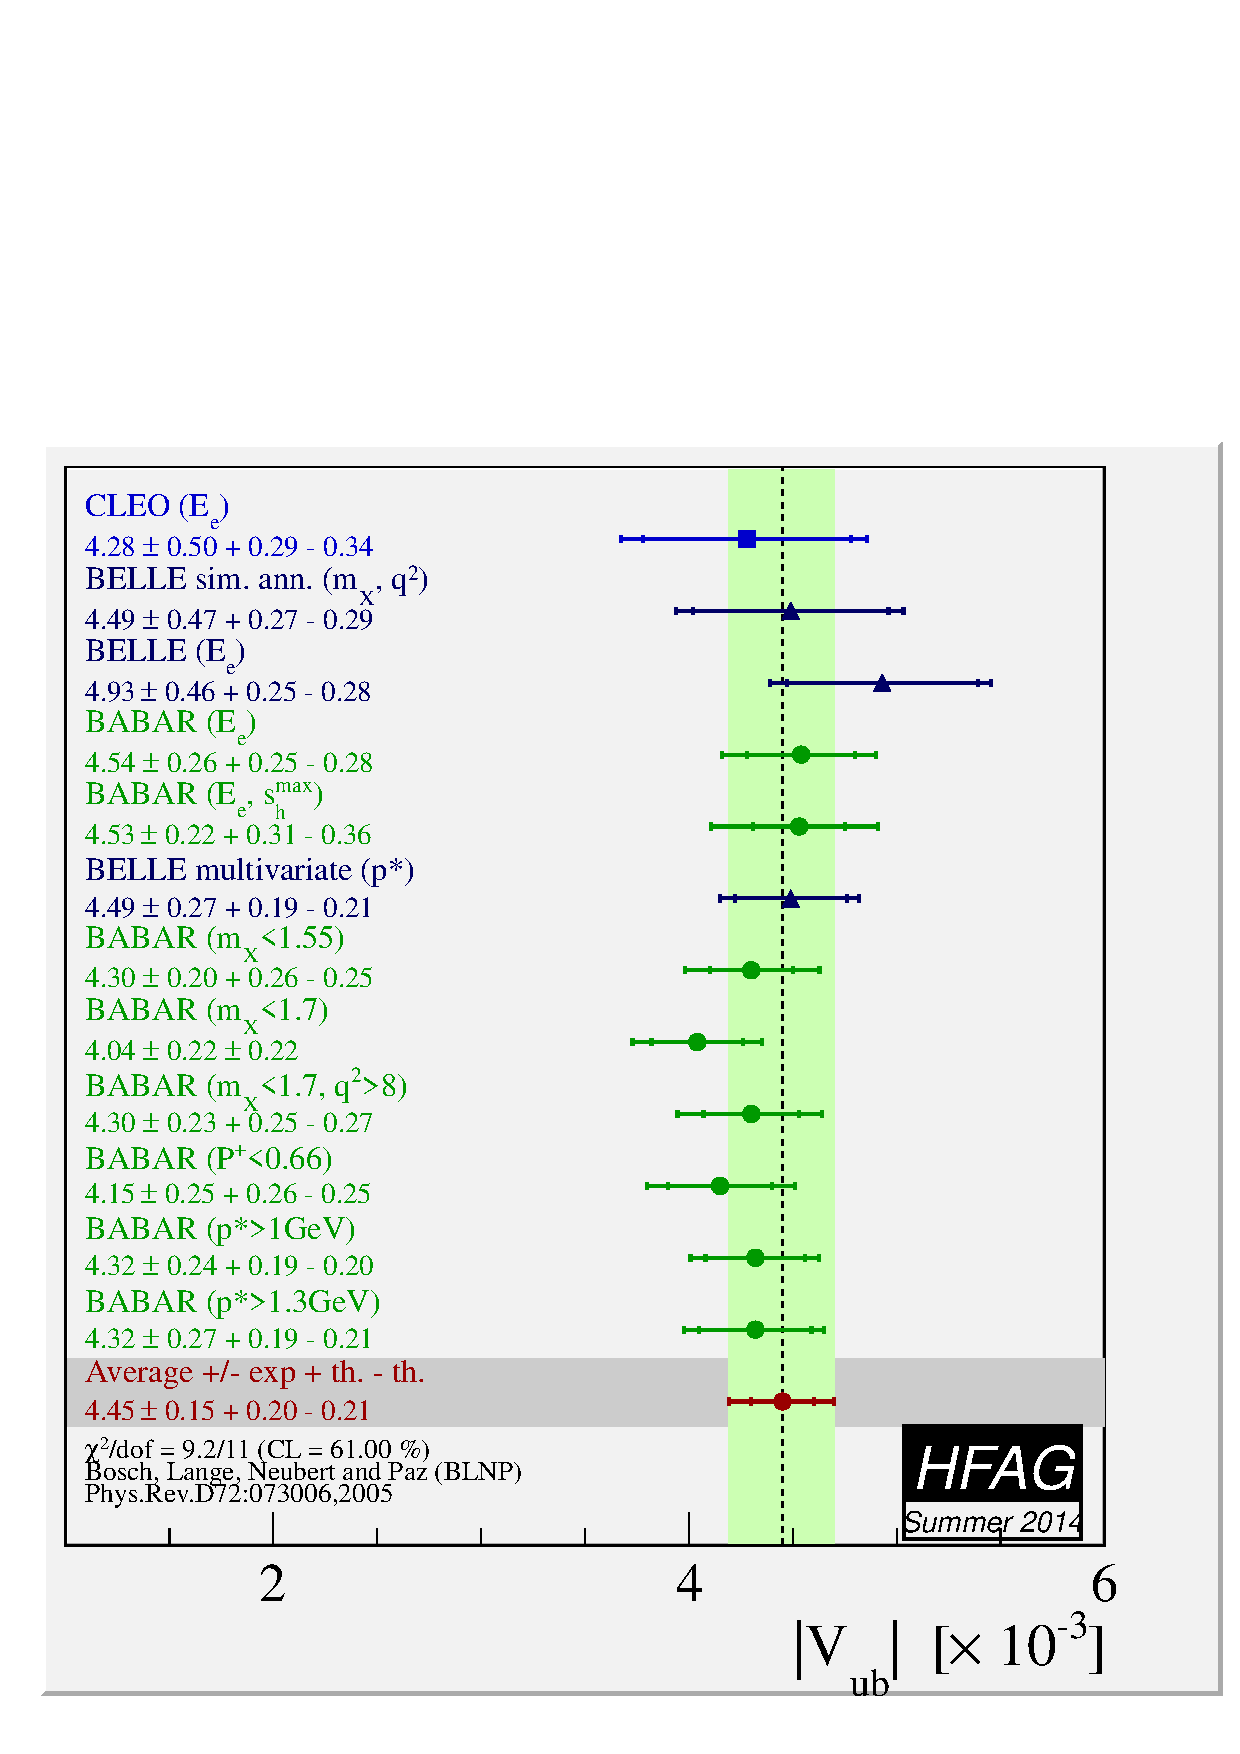
\includegraphics[width=0.48\textwidth]{figures/slb/vub_clnu_mc_twomu_asym_BLNP.pdf}
\end{center}
\caption{Measurements of $\vub$ from inclusive semileptonic decays 
and their average based on the BLNP prescription.
``$E_e$'', ``$M_X$'', ``$(M_X,q^2)$'', ``$P^+$'', ``$p^*$ and ``($E_e,s^{max}_h$)'' indicate the 
distributions and cuts used for the measurement of the partial decay rates.}
\label{fig:BLNP}
\end{figure}

\subsubsection{DGE}
J.R.~Andersen and E.~Gardi (Dressed Gluon Exponentiation, DGE)~\cite{ref:DGE} provide
a framework where the on-shell $b$-quark calculation, converted into hadronic variables, is
directly used as an approximation to the meson decay spectrum without
the use of a leading-power non-perturbative function (or, in other words,
a shape function). The on-shell mass of the $b$-quark within the $B$-meson ($m_b$) is
required as input. 
The DGE calculation uses the $\overline{MS}$ renormalization scheme; the heavy quark parameters determined  
from the global fit in the kinetic scheme, described in \ref{globalfitsKinetic}, were therefore 
translated into the $\overline{MS}$ scheme by using a calculation by Gardi, giving 
$m_b({\overline{MS}})=(4.177 \pm 0.043)$ GeV.
The extracted values
of \vub\, for each measurement along with their average are given in
Table~\ref{tab:bulnu} and illustrated in Figure~\ref{fig:DGE}.
The total error is $^{+4.8}_{-5.0}\%$, whose breakdown is:
statistics ($^{+1.8}_{-1.8}\%$),
detector ($^{+1.7}_{-1.7}\%$),
$B\to X_c \ell^+ \nul$ model ($^{+1.3}_{-1.3}\%$),
$B\to X_u \ell^+ \nul$ model ($^{+2.1}_{-1.9}\%$),
strong coupling $\alpha_s$ ($^{+0.5}_{-0.5}\%$),
$m_b$ ($^{+3.2}_{-3.0}\%$),
%%%%%%%%%%%%%%?!?!?!?spectral fraction ($m_b$) ($^{+3.0}_{-3.3}\%$),
%%%%%%%%%%%%%%?!?!?!?!total semileptonic width ($m_b$) ($^{+3.0}_{-3.0}\%$),
weak annihilation ($^{+0.0}_{-1.9}\%$),
DGE theory: matching scales ($^{+0.5}_{-0.3}\%$).
The largest contribution to the total error is due to the effect of the uncertainty 
on $m_b$. 
%%%%%%%%%%%%%%on the prediction of the event rate, closely followed by the 
%%%%%%%%%%%%%%specific theory error on overall DGE and the total semileptonic decay width.
The uncertainty due to 
weak annihilation has been assumed to be asymmetric, i.e. it only tends to decrease \vub.

\begin{figure}
\begin{center}
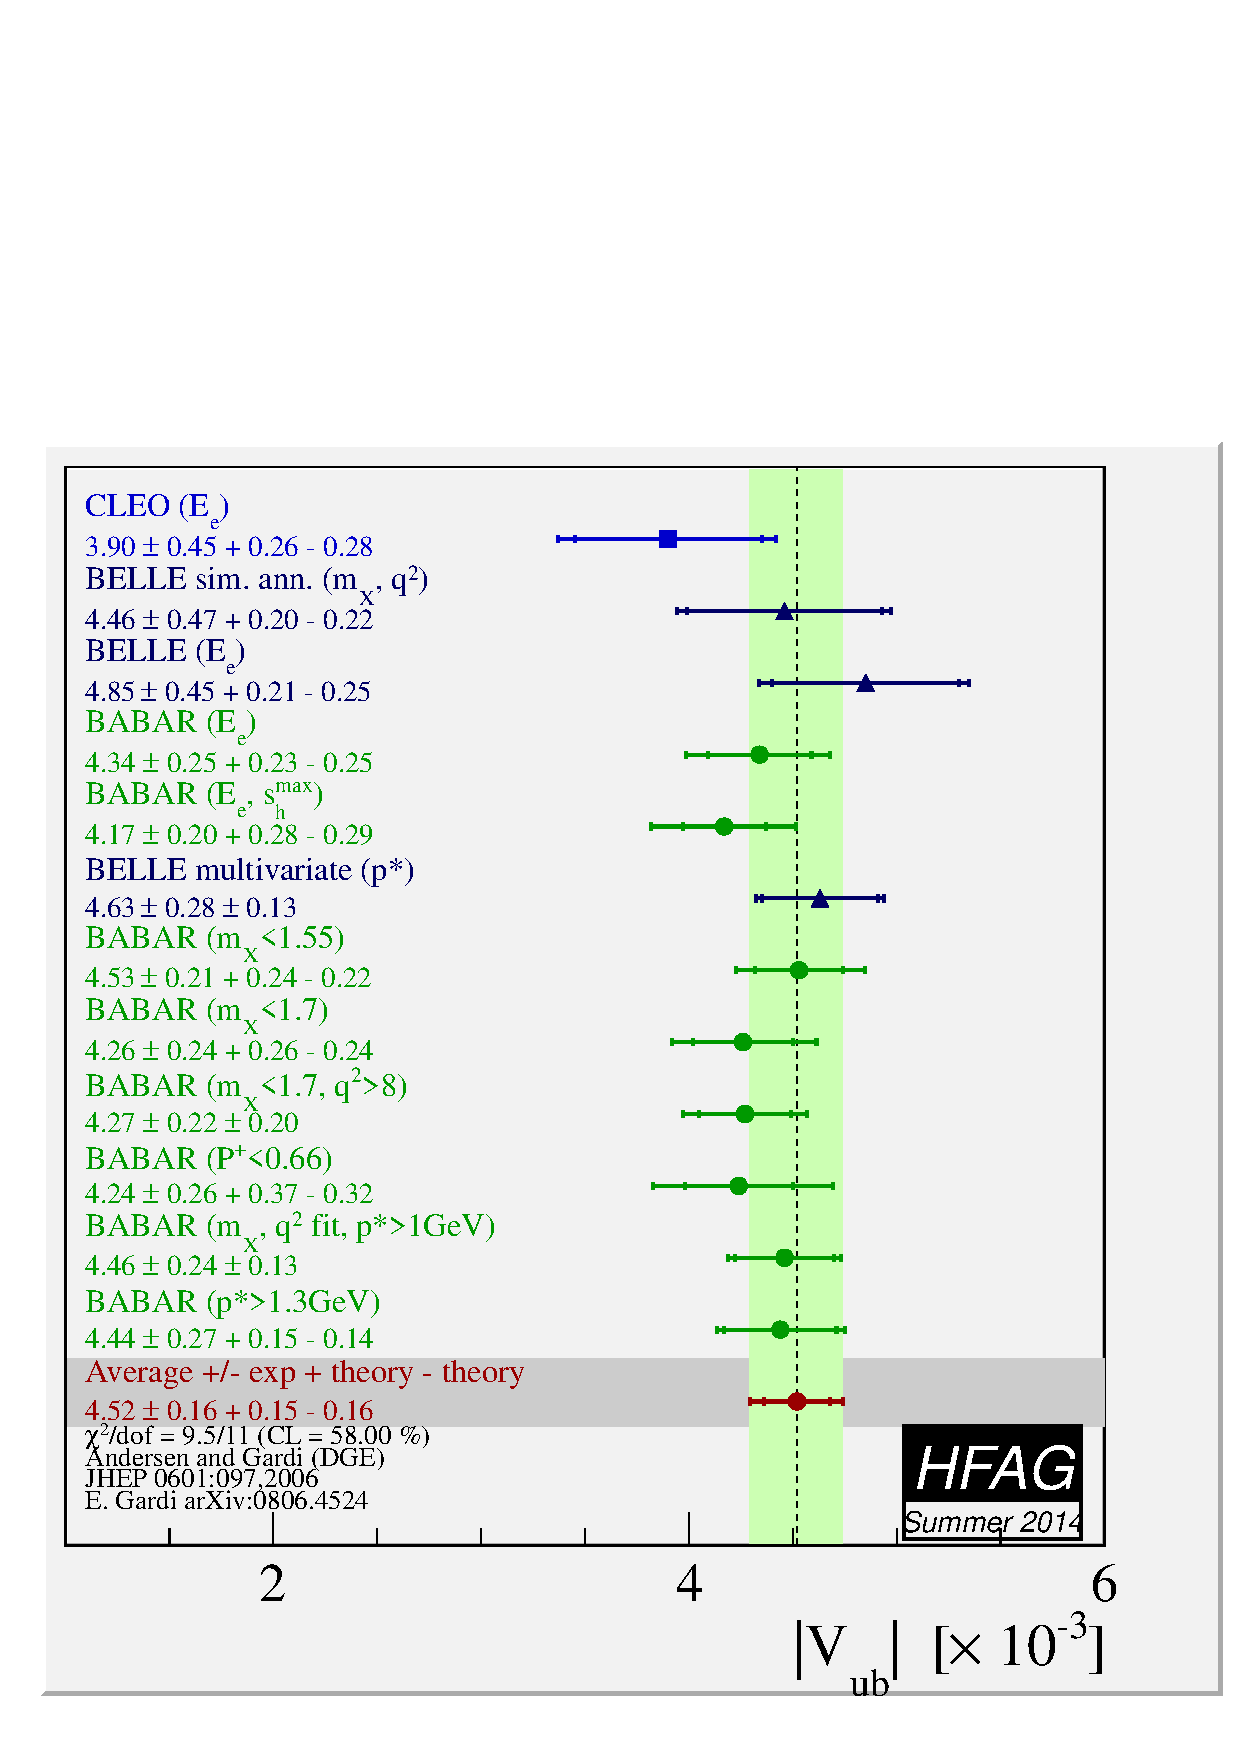
\includegraphics[width=0.48\textwidth]{figures/slb/vub_clnu_mc_asym_DGE.pdf}
\end{center}
\caption{Measurements of $\vub$ from inclusive semileptonic decays 
and their average based on the DGE prescription.
``$E_e$'', ``$M_X$'', ``$(M_X,q^2)$'' `$P^+$'', ``$p^*$ and ``($E_e,s^{max}_h$)'' indicate the 
analysis type and applied cut.}
\label{fig:DGE}
\end{figure}

\subsubsection{GGOU}
Gambino, Giordano, Ossola and Uraltsev (GGOU)~\cite{Gambino:2007rp} 
compute the triple differential decay rates of $B \to X_u \ell^+ \nul$, 
including all perturbative and non--perturbative effects through $O(\alphas^2 \beta_0)$ 
and $O(1/m_b^3)$. 
The Fermi motion is parameterized in terms of a single light--cone function 
for each structure function and for any value of $q^2$, accounting for all subleading effects. 
The calculations are performed in the kinetic scheme, a framework characterized by a Wilsonian 
treatment with a hard cutoff $\mu \sim 1 $ GeV.
GGOU have not included calculations for the ``($E_e,s^{max}_h$)'' analysis. 
The heavy quark parameters determined  
from the global fit in the kinetic scheme, described in \ref{globalfitsKinetic}, are used as inputs: 
$m_b(kin)=(4.541 \pm 0.023)$ GeV, 
$\mu_\pi^2(kin)=(0.414 \pm 0.078)$ GeV$^2$. 
The extracted values
of \vub\, for each measurement along with their average are given in
Table~\ref{tab:bulnu} and illustrated in Figure~\ref{fig:GGOU}.
The total error is $^{+4.3}_{-4.8}\%$ whose breakdown is:
statistics ($^{+1.9}_{-1.9}\%$),
detector ($^{+1.7}_{-1.7}\%$),
$B\to X_c \ell^+ \nul$ model ($^{+1.3}_{-1.3}\%$),
$B\to X_u \ell^+ \nul$ model ($^{+1.9}_{-1.9}\%$),
$\alpha_s$, $m_b$ and other non--perturbative parameters ($^{+1.6}_{-1.6}\%$), 
higher order perturbative and non--perturbative corrections ($^{+1.5}_{-1.5}\%$), 
modelling of the $q^2$ tail and choice of the scale $q^{2*}$ ($^{+1.4}_{-1.4}\%$), 
weak annihilations matrix element ($^{+0.0}_{-2.0}\%$), 
functional form of the distribution functions ($^{+0.2}_{-0.2}\%$), 
The leading uncertainties
on  \vub\ are both from theory, and are due to perturbative and non--perturbative
parameters and the modelling of the $q^2$ tail and choice of the scale $q^{2*}$. 
The uncertainty due to 
weak annihilation has been assumed to be asymmetric, i.e. it only tends to decrease \vub.

\begin{figure}
\begin{center}
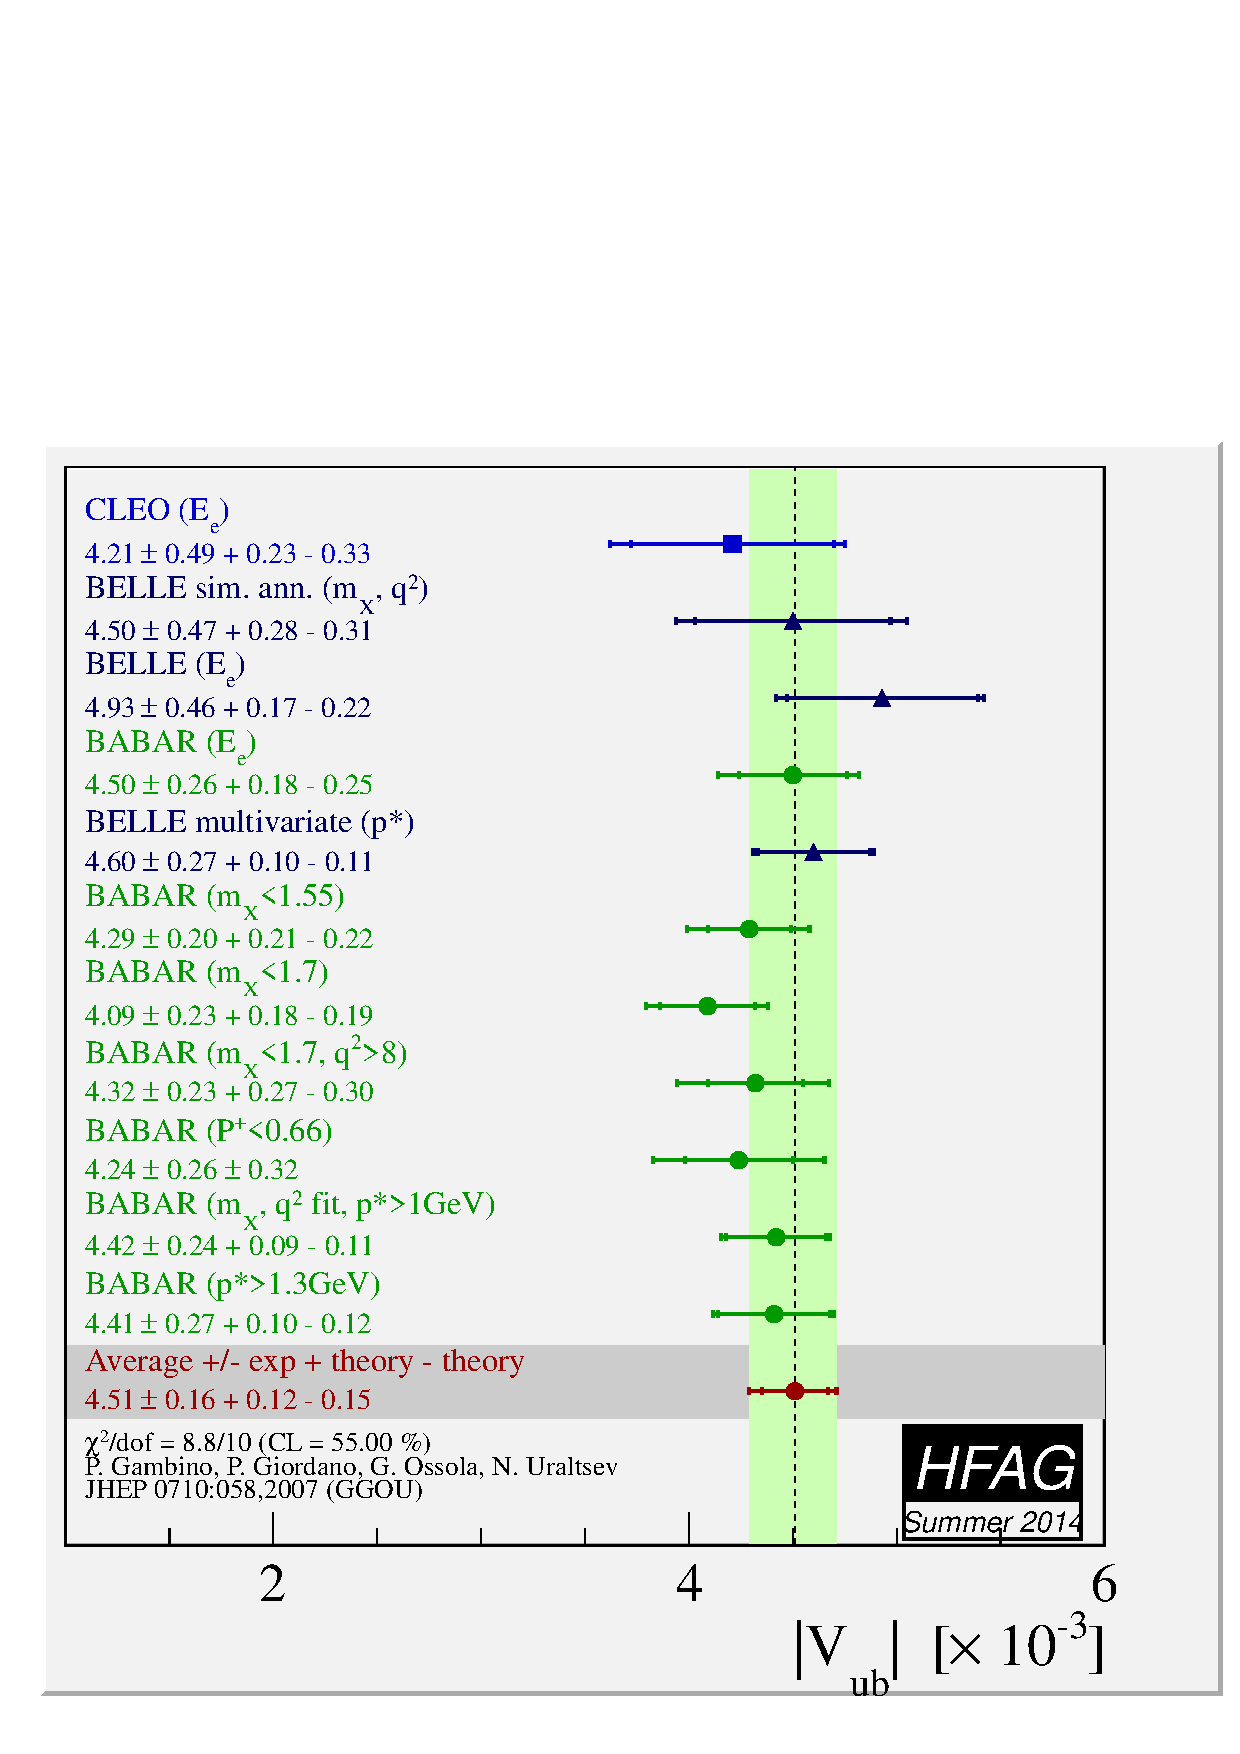
\includegraphics[width=0.48\textwidth]{figures/slb/vub_clnu_mc_GGOU.pdf}
\end{center}
\caption{Measurements of $\vub$ from inclusive semileptonic decays 
and their average based on the GGOU prescription.
``$E_e$'', ``$M_X$'', ``$(M_X,q^2)$'' `$P^+$'', ``$p^*$ and ``($E_e,s^{max}_h$)''  indicate the
analysis type and applied cut.}
\label{fig:GGOU}
\end{figure}

\subsubsection{ADFR}
Aglietti, Di Lodovico, Ferrera and Ricciardi (ADFR)~\cite{Aglietti:2007ik}
use an approach to extract \vub, which makes use of the ratio
of the  $B \to X_c \ell^+ \nul$ and $B \to X_u \ell^+ \nul$ widths. 
The normalized triple differential decay rate for 
$B \to X_u \ell^+ \nul$~\cite{Aglietti:2006yb,Aglietti:2005mb, Aglietti:2005bm, Aglietti:2005eq}
is calculated with a model based on (i) soft--gluon resummation 
to next--to--next--leading order and (ii) an effective QCD coupling without
Landau pole. This coupling is constructed by means of an extrapolation to low
energy of the high--energy behaviour of the standard coupling. More technically,
an analyticity principle is used.
The lower cut on the electron energy for the endpoint analyses is 2.3~GeV~\cite{Aglietti:2006yb}.
The ADFR calculation uses the $\overline{MS}$ renormalization scheme; the heavy quark parameters determined  
from the global fit in the kinetic scheme, described in \ref{globalfitsKinetic}, were therefore 
translated into the $\overline{MS}$ scheme by using a calculation by Gardi, giving 
$m_b({\overline{MS}})=(4.177 \pm 0.043)$ GeV.
The extracted values
of \vub\, for each measurement along with their average are given in
Table~\ref{tab:bulnu} and illustrated in Figure~\ref{fig:AC}.
The total error is $^{+5.4}_{-5.3}\%$ whose breakdown is:
statistics ($^{+1.8}_{-1.8}\%$),
detector ($^{+1.8}_{-2.0}\%$),
$B\to X_c \ell^+ \nul$ model ($^{+1.4}_{-1.4}\%$),
$B\to X_u \ell^+ \nul$ model ($^{+1.3}_{-1.3}\%$),
$\alpha_s$ ($^{+1.1}_{-1.0}\%$), 
$|V_{cb}|$ ($^{+2.0}_{-2.0}\%$), 
$m_b$ ($^{+0.7}_{-0.7}\%$), 
$m_c$ ($^{+0.4}_{-0.7}\%$), 
semileptonic branching fraction ($^{+0.8}_{-0.7}\%$), 
theory model ($^{+3.5}_{-3.5}\%$).
The leading
uncertainty, from theory, is due to the theory model.

\begin{figure}
\begin{center}
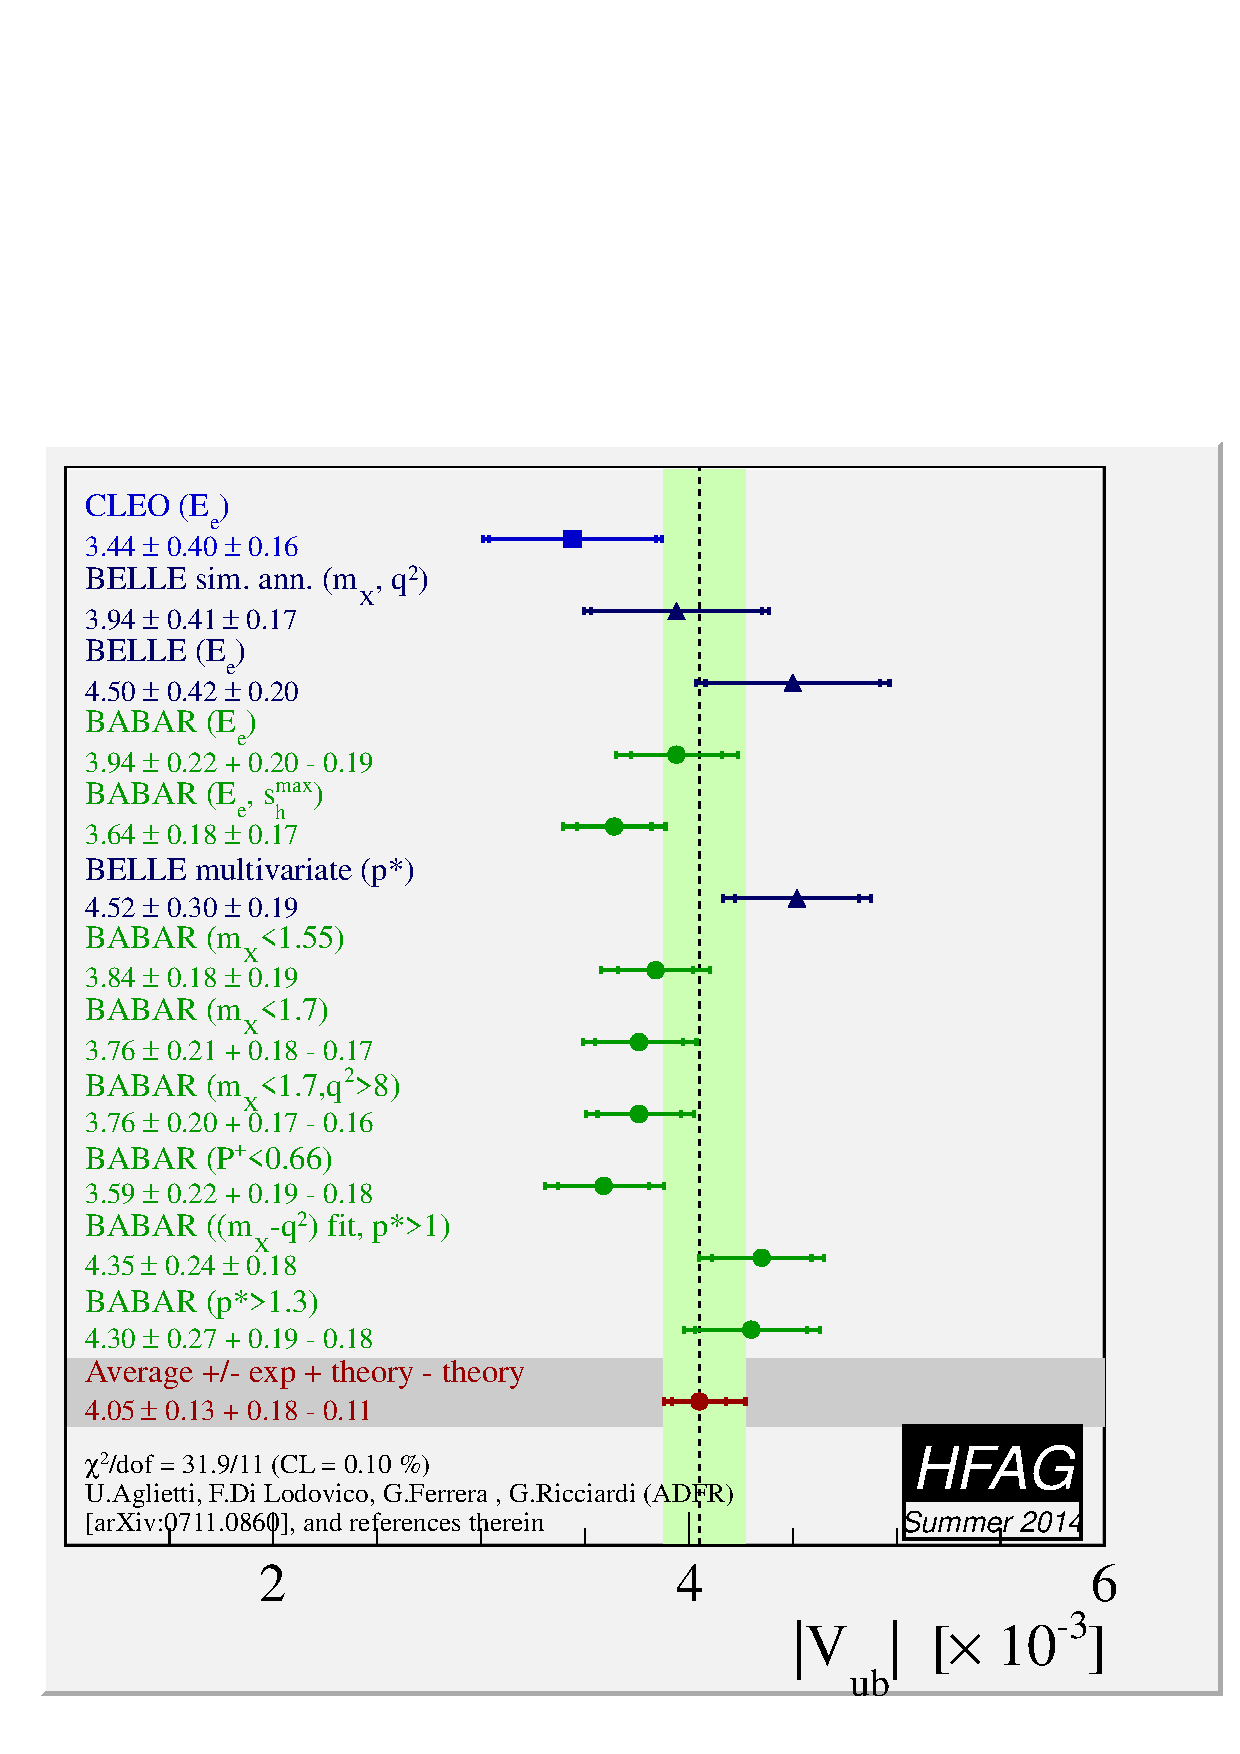
\includegraphics[width=0.48\textwidth]{figures/slb/vub_clnu_mc_ADFR.pdf}
\end{center}
\caption{Measurements of $\vub$ from inclusive semileptonic decays 
and their average based on the ADFR prescription.
``$E_e$'', ``$M_X$'', ``$(M_X,q^2)$'' `$P^+$'', ``$p^*$ and ``($E_e,s^{max}_h$)'' indicate the 
analysis type and applied cut.}
\label{fig:AC}
\end{figure}



\subsubsection{BLL}
Bauer, Ligeti, and Luke (BLL)~\cite{ref:BLL} give a
HQET-based prescription that advocates combined cuts on the dilepton invariant mass, $q^2$,
and hadronic mass, $m_X$, to minimise the overall uncertainty on \vub.
In their reckoning a cut on $m_X$ only, although most efficient at
preserving phase space ($\sim$80\%), makes the calculation of the partial
rate untenable due to uncalculable corrections
to the $b$-quark distribution function or shape function. These corrections are
suppressed if events in the low $q^2$ region are removed. The cut combination used
in measurements is $M_x<1.7$ GeV/$c^2$ and $q^2 > 8$ GeV$^2$/$c^2$.  
The extracted values
of \vub\, for each measurement along with their average are given in
Table~\ref{tab:bulnu} and illustrated in Figure~\ref{fig:BLL}.
The total error is $^{+7.7}_{-7.7}\%$ whose breakdown is:
statistics ($^{+3.3}_{-3.3}\%$),
detector ($^{+3.0}_{-3.0}\%$),
$B\to X_c \ell^+ \nul$ model ($^{+1.6}_{-1.6}\%$),
$B\to X_u \ell^+ \nul$ model ($^{+1.1}_{-1.1}\%$),
spectral fraction ($m_b$) ($^{+3.0}_{-3.0}\%$),
perturbative : strong coupling $\alpha_s$ ($^{+3.0}_{-3.0}\%$),
residual shape function ($^{+2.5}_{-2.5}\%$),
third order terms in the OPE ($^{+4.0}_{-4.0}\%$),
The leading
uncertainties, both from theory, are due to residual shape function
effects and third order terms in the OPE expansion. The leading
experimental uncertainty is due to statistics. 

\begin{figure}
\begin{center}
%\includegraphics[width=0.48\textwidth]{figures/slb/vub_mxq2_allMoments.eps}
\end{center}
\caption{Measurements of $\vub$ from inclusive semileptonic decays 
and their average in the BLL prescription.
``$(M_X, q^2)$'' indicates the analysis type.}
\label{fig:BLL}
\end{figure}


\subsubsection{Summary}
A summary of the averages presented in several different
frameworks and results by V.B.~Golubev, V.G.~Luth and Yu.I.~Skovpen~\cite{Golubev:2007cs},
based on prescriptions by LLR~\cite{Leibovich:1999xf} and LNP~\cite{Lange:2005qn} 
to reduce the leading shape function uncertainties are presented in 
Table~\ref{tab:vubcomparison}.
A value judgement based on a direct comparison should be
avoided at the moment, experimental and theoretical uncertainties play out
differently between the schemes and the theoretical assumptions for the
theory calculations are different.

\begin{table}[!htb]
\caption{\label{tab:vubcomparison}
Summary of inclusive determinations of $\vub$.
The errors quoted on \vub\ correspond to experimental and theoretical uncertainties, except for the last two 
measurements where the errors are due to the \babar\ endpoint analysis, the \babar $b\to s\gamma$ analysis~\cite{Aubert:2006qi}, 
the theoretical errors and $V_{ts}$ for the last averages. 
}
\begin{center}
\begin{small}
\begin{tabular}{|lc|}
\hline
Framework
&  $\Vub [10^{-3}]$\\
\hline\hline
BLNP
& $4.45 \pm 0.15 ^{+0.20}_{-0.21}$ \\ 
DGE
& $4.52 \pm 0.16 ^{+0.15}_{-0.16}$ \\
GGOU
& $4.51 \pm 0.16 ^{+0.12}_{-0.15}$ \\
ADFR
& $4.05 \pm 0.13 ^{+0.18}_{-0.11}$ \\
BLL ($m_X/q^2$ only)
& $4.62 \pm 0.20 \pm 0.29$ \\ 
LLR (\babar)~\cite{Aubert:2006qi}
& $4.43 \pm 0.45 \pm 0.29$ \\
LLR (\babar)~\cite{Golubev:2007cs}
& $4.28 \pm 0.29 \pm 0.29 \pm 0.26 \pm0.28$ \\
LNP (\babar)~\cite{Golubev:2007cs}
& $4.40 \pm 0.30 \pm 0.41 \pm 0.23$ \\
\hline
\end{tabular}\\
\end{small}
\end{center}
\end{table}






